\chapter{Training}


\section{Activation Functions}
\label{sec:activation}
\subsection{Initial \& Convolutional Layers}
At the end of each transition, an elementwise activation function is applied 
following completion of all computations, including multiplication by the 
relevant weight matrix.  For all but the final layer, that function is 
ReLU\cite{nair2010rectified}, defined in figure \ref{fig:relu}.

\begin{figure}[h]
	\centering
	\begin{minipage}{.48\textwidth}
		\begin{equation*}
			relu(x) = \begin{cases}
				0 & x < 0\\
				x & x \geq 0
			\end{cases}
		\end{equation*}
	\end{minipage}
	\begin{minipage}{.48\textwidth}
		\resizebox{\textwidth}{!}{
		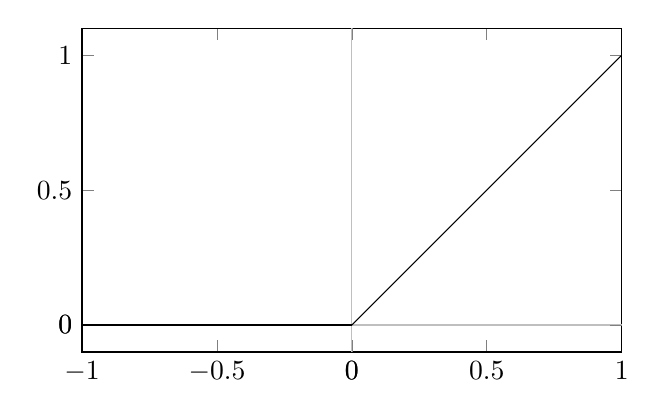
\begin{tikzpicture}
			\begin{axis}[domain=-1:1, unit vector ratio*=1 1 1,
					enlarge x limits=false, extra y ticks=0, extra x ticks=0,
					extra tick style={grid=major}]
				\addplot[color=black][domain=0:1] {x} [mark=none, smooth];
				\addplot[color=black][domain=-1:0] {0} [mark=none smooth];
			\end{axis}
		\end{tikzpicture}
		}
	\end{minipage}
	\caption{ReLU function definition and graph}
	\label{fig:relu}
\end{figure}\noindent


\subsection{Final Layer}
\label{subsec:finalactivation}
ReLU's preservation of positive values and elimination of negative values work 
in concert with the activation function of the final layer, hyperbolic tangent 
(\figref{fig:tanh}).
The clipping of negative values to 0 in previous layers of the network allows 
greater imprecision in the penultimate layer in order to predict a 0 in the 
output adjacency matrix: rather than needing to fine tune the filters to produce 
exactly 0 for nonexistent connections, the model need only drive the values for 
such neuron pairs into the negatives, and let the application of ReLU correct.  

\begin{wrapfigure}[5]{r}{.45\textwidth}
	\centering
	\vspace{-14pt}
	\resizebox{.43\textwidth}{!}{
		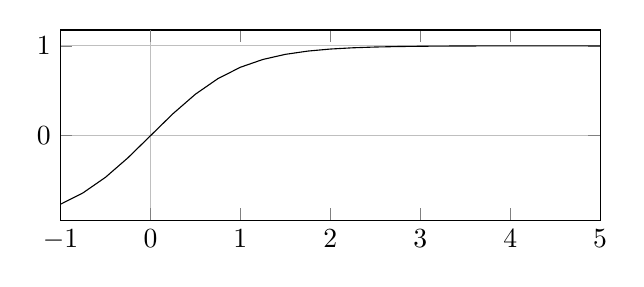
\begin{tikzpicture}
			\begin{axis}[domain=-1:5, unit vector ratio*=1 1 1,
				ytick={0,1}, enlarge x limits=false, ymajorgrids,
				xtick={-1,1,2,3,4,5},
				extra x ticks=0, extra tick style={grid=major}]
				\addplot[color=black] {tanh(x)} [mark=none, smooth];
			\end{axis}
		\end{tikzpicture}
	}
	\caption{Graph of $y=\tanh(x)$}
	\label{fig:tanh}
\end{wrapfigure}
Similarly, the final layer \textit{tanh} allows the network to drive weights for 
probable connections far into the positives, with the activation function 
ultimately mapping large values into a small range closely approaching 1.

\section{Loss \& Optimization}
\label{sec:lossandop}
In a nutshell, backpropagation via gradient descent is a method for training 
neural networks by calculating the extent to which each value in a particular 
layer is responsible for the overall network error on a single data point or 
batch, then correcting that value by an amount commensurate to its error and 
overall learning rate. This process operates from the final layer back to the 
first, hence `backpropagation'.\cite{Rumelhart}

In order to effectively descend the gradient, a network needs a function 
defining error from the desired output and an algorithm for applying gradient 
descent based on that error and a specified learning rate.

The loss function must provide useful values to the optimizer in order to allow 
effective gradient descent towards the goal, and the optimizer must adjust the 
network fast enough to converge to the target while avoiding converging to a 
suboptimal solution. As the network gets closer to an optimal state, adjusting 
at the same rate as at the start of training will almost invariably overshoot 
the desired configuration. Due to this, the optimizer must dynamically modify 
the extent to which it adjusts the network as training goes on.

\subsection{Loss Function}
% why was this so goddamn hard
\edef\myindent{\the\parindent}
\begin{minipage}{\textwidth}\setlength{\parindent}{\myindent}
\noindent We define a basic custom loss function in order to better fit the 
outputs we expect to see.

For final model output $\mathbb{O}$ and target $\mathbb{T}$, we take the sum 
squared difference, $S$, of the two vectors and the sum over $\mathbb{T}$, 
$S_T$, \eqref{eq:ssd}, and divide these two values to achieve loss 
$L$.\footnotemark
\end{minipage}
\begin{subequations}
	\centering
	\begin{align}
		S &= \sum_i \left(\mathbb{O}_i - \mathbb{T}_i \right)^2
		= \sum_i \left[\left(\mathbb{O} - \mathbb{T})_i \right)\right]^2 &
		S_T &= \sum_i \mathbb{T}_i
		\label{eq:ssd}
	\end{align}
	\begin{equation}
		L = \frac{S}{S_T}
		\label{eq:los}
	\end{equation}
	\label{eq:losscalc}
\end{subequations}

\footnotetext{Recall from \ref{subsubsec:targetdata} that the targets 
$\mathbb{T}$ given to the model are the flattend generator adjacency matrix; 
dimensionality $(1 \times n^2)$.}
Thus, rather than scale loss with the number of total possible connections 
($n^2$) as with a mean squared error, we scale our loss with the number of 
actual connections in the true adjacency matrix, keeping the loss values 
somewhat higher in the early stages of training, yet still falling to levels 
comparable to that of MSE as the model learns to predict appropriately.

%\begin{minipage}{\textwidth}
\subsubsection{Effects}
\label{subsubsec:losseffects}
\begin{wraptable}[5]{r}{.3\textwidth}
	\captionsetup{justification=centering}
	\vspace{-15pt}
	\centering
	\adjacencyT{0 & 0 & 0}{1 & 0 & 0}{1 & 1 & 0}
	\vspace{-5pt}
	\captionof{figure}{\linespread{1.2}\selectfont{}Example adjacency matrix}
	\label{fig:loss_ex}
\end{wraptable}
Consider a model analyzing data from a 3-node generator with an adjacency matrix 
as given in \figref{fig:loss_ex}, and suppose that its output is a vector 
containing two correct values and one wrong value.  Then our parameters for 
determining loss by way of \eqref{eq:losscalc} are as follows:
\begin{align*}
	\mathbb{O} &= \begin{bmatrix} 0.0 & 0.0 & 0.0 & 1.0 & 0.0 & 0.0 & 1.0 & 0.0 
			   & 1.0\end{bmatrix}\\
	\mathbb{T} &= \begin{bmatrix} 0.0 & 0.0 & 0.0 & 1.0 & 0.0 & 0.0 & 1.0 & 1.0 
				& 0.0\end{bmatrix}\\
	\left(\mathbb{O} - \mathbb{T}\right)^2 &= \begin{bmatrix} 0.0 & 0.0 & 0.0 & 
		0.0 & 0.0 & 0.0 & 0.0 & 1.0 & 1.0\end{bmatrix}\\
	S 	&= \sum_i \left(\mathbb{O}_i - \mathbb{T}_i \right)^2 = 2.0\\
	S_T &= \sum_i \mathbb{T}_i = 3.0
	\intertext{And our loss is finally determined:}
	L 	&= \frac{S}{S_T} = \frac{2.0}{3.0} = .\overline{6}
\end{align*}
%\end{minipage}
Thus, our loss function `punishes' the network equally for false positives and 
false negatives: due to the squared difference, a 1 where there should be a 0 
adds the same loss as a 0 where there should be a one. This is perhaps not the 
ideal method; see \ref{subsec:lossdisc}. The value produced for each 
input/target pair is then passed to the optimizer.

\subsection{Optimizer Function}
\label{subsec:optimizer}
We used the Adam optimizer as provided by 
TensorFlow\cite{tensorflow2015-whitepaper}, providing different initial learning 
rates per dataset. Those values were arrived at via experimentation. After 
initializing the optimizer, it is passed the loss at each step and performs 
gradient descent on the trainable matrices.

Adam adjusts its learning rate as time goes on, according to the following 
equation, where $\beta_n^t$ indicates exponentiation by $t$ and $lr$ denotes 
learning rate:
\begin{figure}[h]
	\begin{minipage}[b]{.38\textwidth}
		\centering
		\begin{gather}
			\nonumber
			\beta_1 = 0.9\\
			\nonumber
			\beta_2 = 0.999\\
			\nonumber
			lr_t = lr_{init} \times \frac{\sqrt{1-\beta_2^t}}{1-\beta_1^t}
		\end{gather}
	\end{minipage}
	\hfill
	\begin{minipage}{.6\textwidth}
		\centering
		\resizebox{\textwidth}{!}{
			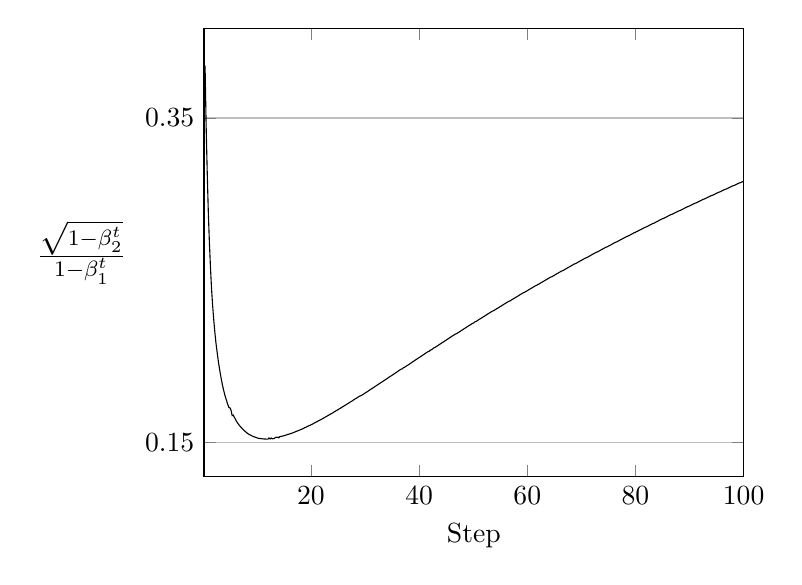
\begin{tikzpicture}
			\begin{axis}[domain=.01:100, ytick={0,.15,.35}, samples=500,
				ylabel=$\frac{\sqrt{1-\beta_2^t}}{1-\beta_1^t}$,
				ylabel style={rotate=-90, font=\large},
					enlarge x limits=false, ymajorgrids, extra x ticks=0,
					extra tick style={grid=major}, xlabel=Step]
					\addplot[color=black] {sqrt(1-.999^x)/(1-.9^x)} [mark=none, 
			smooth];
			\end{axis}
		\end{tikzpicture}
		}
		\captionof{figure}{Adam decay function over 100 steps. Converges 
			asymptotically to 1.}
	\end{minipage}
\end{figure}


\section{Matrices}
\subsection{Initialization}
Initially, we seeded our matrices with random values from a normal distribution 
of standard deviation 1.0 and mean 0, using the TensorFlow implementation of 
\texttt{tf.random\_normal(<dimensions>)}. Due, however, to the cumulative nature 
of our matrix operations (in the locality layer, for instance, there are three 
separate multiplications (\ref{subsubsec:matconvlayer})), we found that the 
values of the outputs were so high or low as to render the model somewhat random 
in its convergence, or lack thereof.

We found that by reducing the standard deviation of our distributions to 0.25, 
we can ensure that most, if not all, training runs of our model converge. If 
raised higher, models trained on complex generator networks may consistently 
fail to converge, and a lower value tends to lead to convergence on non-optimal 
solutions, such as prediciting all zeroes. 

\subsection{Locality Layer Operations}
\label{subsec:localops}
As discussed in \ref{subsubsec:locality}, a different method for integrating 
inputs and outputs to a given edge was originally considered. If $\mathbb{I}$ is 
the average input vector for some edge $d_{ij}$, and $\mathbb{O}$ is the average 
output vector, then the original operations went as follows:
\begin{subequations}
\begin{align}
	\underset{d \times 1}{\mathbb{I_D}} &= \underset{d \times 
	2d}{\mathbb{W}_{in}^\prime} \times 
	\left(\frac{\mathbb{I}}{d_{ij}^\prime}\right) &
	\underset{d \times 1}{\mathbb{O_D}} &= \underset{d \times 
		2d}{\mathbb{W}_{out}^\prime} \times 
		\left(\frac{d_{ij}^\prime}{\mathbb{O}}\right)
\end{align}
\begin{equation}
		d_{ij}^{\prime\prime} = \mathbb{I_D} + \mathbb{O_D}
\end{equation}
\end{subequations}
This was suboptimal for a variety of reasons. The addition of the two vectors in 
the final step implied that both inputs and outputs were of exactly equal value 
in determining the existence of an edge, and even further that, for any index 
into those two vectors, the values at that index would be usefully comparable in 
some way.

Beyond this, the integration of locality data in this format seemed to require 
careful tuning, and gradient descent did not work well with this setup.  
Specifically, at an initial network state, the first layer has not been 
optimized to provide useful data targeted at the second layer summations that 
produce $\mathbb{I}$ and $\mathbb{O}$. However, the only reason for the network 
to trend towards this type of data shaping in the first layer would be an 
observed decrease in loss. While doubtless possible, it seems a more attractive 
(loss optimizing) option appears: zero the left side of 
$\mathbb{W}_{in}^\prime$, and the right of $\mathbb{W}_{out}^\prime$. As the 
noisy locality data is removed from the system, the loss decreases, and 
eventually the network arrives at a somewhat remarkable state: the halves of the 
weight matrices that remain in use converge to the same values, operating as 
they are on the same data.

For these reasons, we opted for the implementation described in 
\ref{subsubsec:locality}, in which we force the integration of locality data 
into the model's calculations via entrywise multiplication, and provide an 
optimizable matrix for combining input and output data, allowing the network to 
learn which parts are most important.

\section{Hyperparameter Optimization}
\subsection{Batch Size}
`Batching' refers to the process of assembling a set of items from the training 
data and passing them through the network in parallel, then optimizing over the 
resulting losses simultaneously. This greatly speeds computation speed by 
removing the costly optimization operation from each step. We found that 32 
units per batch was an effective number, offering high training speeds with 
relatively stable loss curves.
